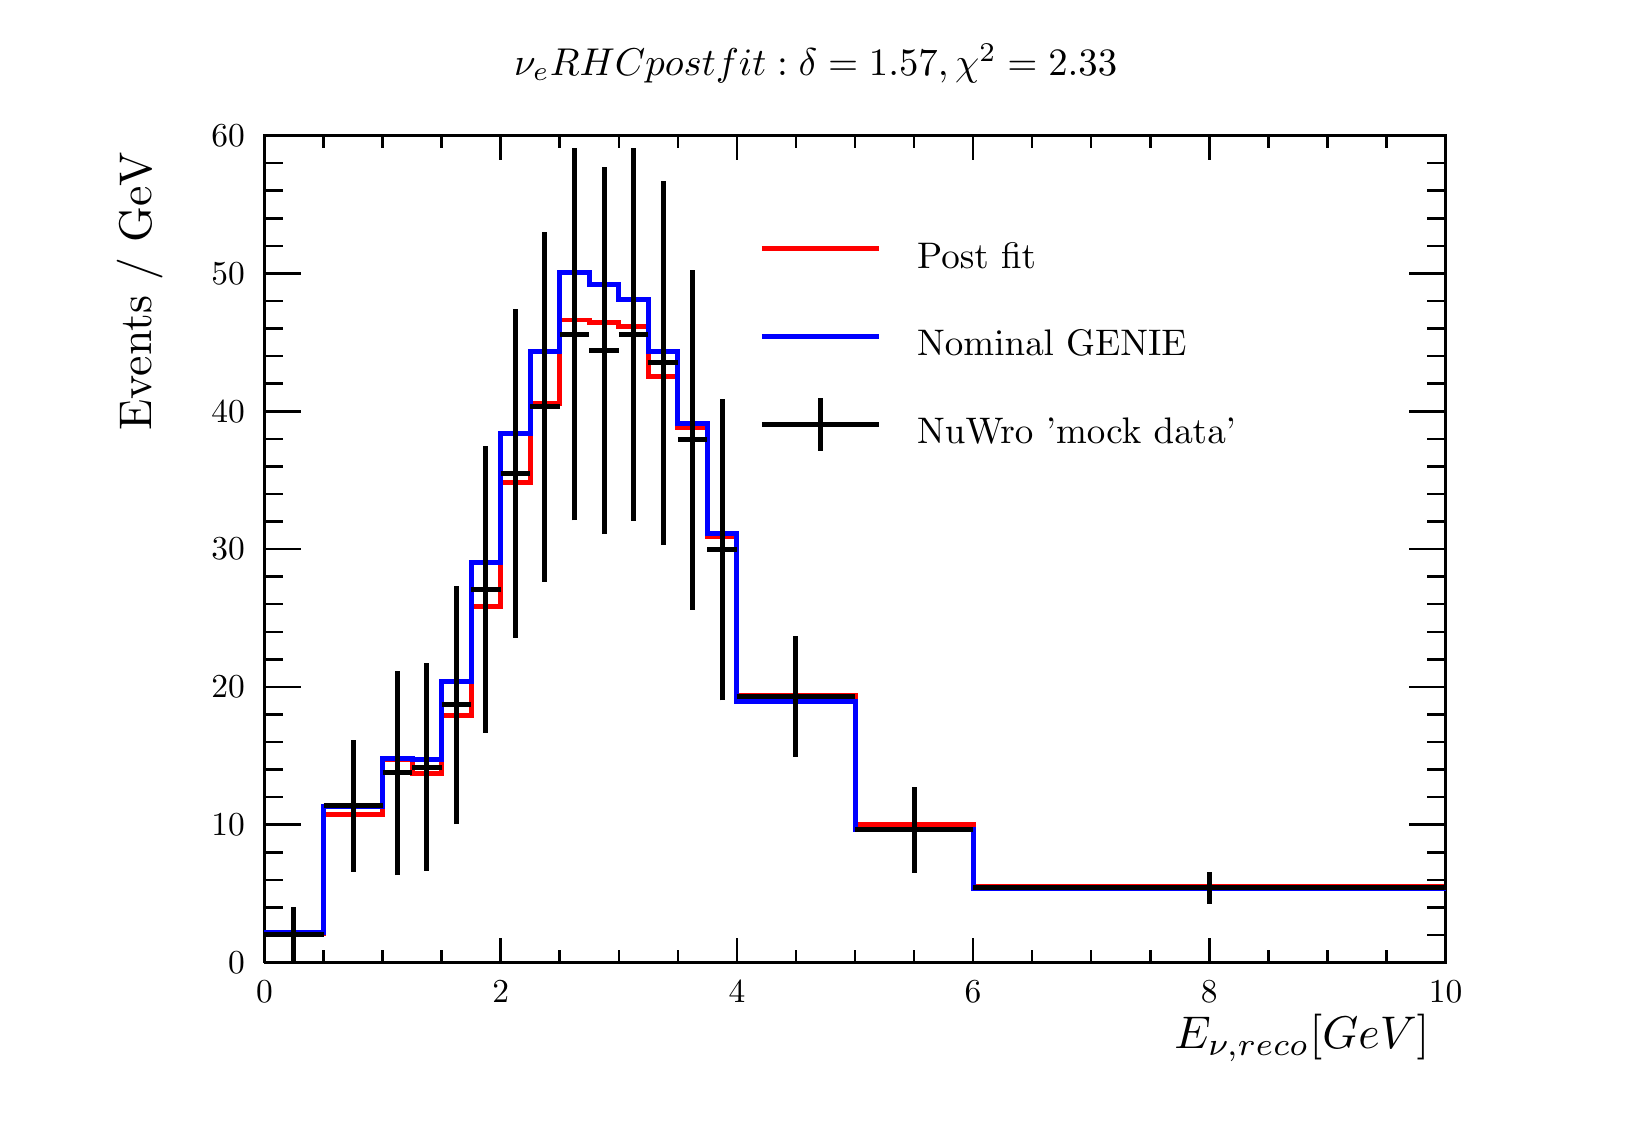
\begin{tikzpicture}
\pgfdeclareplotmark{cross} {
\pgfpathmoveto{\pgfpoint{-0.3\pgfplotmarksize}{\pgfplotmarksize}}
\pgfpathlineto{\pgfpoint{+0.3\pgfplotmarksize}{\pgfplotmarksize}}
\pgfpathlineto{\pgfpoint{+0.3\pgfplotmarksize}{0.3\pgfplotmarksize}}
\pgfpathlineto{\pgfpoint{+1\pgfplotmarksize}{0.3\pgfplotmarksize}}
\pgfpathlineto{\pgfpoint{+1\pgfplotmarksize}{-0.3\pgfplotmarksize}}
\pgfpathlineto{\pgfpoint{+0.3\pgfplotmarksize}{-0.3\pgfplotmarksize}}
\pgfpathlineto{\pgfpoint{+0.3\pgfplotmarksize}{-1.\pgfplotmarksize}}
\pgfpathlineto{\pgfpoint{-0.3\pgfplotmarksize}{-1.\pgfplotmarksize}}
\pgfpathlineto{\pgfpoint{-0.3\pgfplotmarksize}{-0.3\pgfplotmarksize}}
\pgfpathlineto{\pgfpoint{-1.\pgfplotmarksize}{-0.3\pgfplotmarksize}}
\pgfpathlineto{\pgfpoint{-1.\pgfplotmarksize}{0.3\pgfplotmarksize}}
\pgfpathlineto{\pgfpoint{-0.3\pgfplotmarksize}{0.3\pgfplotmarksize}}
\pgfpathclose
\pgfusepathqstroke
}
\pgfdeclareplotmark{cross*} {
\pgfpathmoveto{\pgfpoint{-0.3\pgfplotmarksize}{\pgfplotmarksize}}
\pgfpathlineto{\pgfpoint{+0.3\pgfplotmarksize}{\pgfplotmarksize}}
\pgfpathlineto{\pgfpoint{+0.3\pgfplotmarksize}{0.3\pgfplotmarksize}}
\pgfpathlineto{\pgfpoint{+1\pgfplotmarksize}{0.3\pgfplotmarksize}}
\pgfpathlineto{\pgfpoint{+1\pgfplotmarksize}{-0.3\pgfplotmarksize}}
\pgfpathlineto{\pgfpoint{+0.3\pgfplotmarksize}{-0.3\pgfplotmarksize}}
\pgfpathlineto{\pgfpoint{+0.3\pgfplotmarksize}{-1.\pgfplotmarksize}}
\pgfpathlineto{\pgfpoint{-0.3\pgfplotmarksize}{-1.\pgfplotmarksize}}
\pgfpathlineto{\pgfpoint{-0.3\pgfplotmarksize}{-0.3\pgfplotmarksize}}
\pgfpathlineto{\pgfpoint{-1.\pgfplotmarksize}{-0.3\pgfplotmarksize}}
\pgfpathlineto{\pgfpoint{-1.\pgfplotmarksize}{0.3\pgfplotmarksize}}
\pgfpathlineto{\pgfpoint{-0.3\pgfplotmarksize}{0.3\pgfplotmarksize}}
\pgfpathclose
\pgfusepathqfillstroke
}
\pgfdeclareplotmark{newstar} {
\pgfpathmoveto{\pgfqpoint{0pt}{\pgfplotmarksize}}
\pgfpathlineto{\pgfqpointpolar{44}{0.5\pgfplotmarksize}}
\pgfpathlineto{\pgfqpointpolar{18}{\pgfplotmarksize}}
\pgfpathlineto{\pgfqpointpolar{-20}{0.5\pgfplotmarksize}}
\pgfpathlineto{\pgfqpointpolar{-54}{\pgfplotmarksize}}
\pgfpathlineto{\pgfqpointpolar{-90}{0.5\pgfplotmarksize}}
\pgfpathlineto{\pgfqpointpolar{234}{\pgfplotmarksize}}
\pgfpathlineto{\pgfqpointpolar{198}{0.5\pgfplotmarksize}}
\pgfpathlineto{\pgfqpointpolar{162}{\pgfplotmarksize}}
\pgfpathlineto{\pgfqpointpolar{134}{0.5\pgfplotmarksize}}
\pgfpathclose
\pgfusepathqstroke
}
\pgfdeclareplotmark{newstar*} {
\pgfpathmoveto{\pgfqpoint{0pt}{\pgfplotmarksize}}
\pgfpathlineto{\pgfqpointpolar{44}{0.5\pgfplotmarksize}}
\pgfpathlineto{\pgfqpointpolar{18}{\pgfplotmarksize}}
\pgfpathlineto{\pgfqpointpolar{-20}{0.5\pgfplotmarksize}}
\pgfpathlineto{\pgfqpointpolar{-54}{\pgfplotmarksize}}
\pgfpathlineto{\pgfqpointpolar{-90}{0.5\pgfplotmarksize}}
\pgfpathlineto{\pgfqpointpolar{234}{\pgfplotmarksize}}
\pgfpathlineto{\pgfqpointpolar{198}{0.5\pgfplotmarksize}}
\pgfpathlineto{\pgfqpointpolar{162}{\pgfplotmarksize}}
\pgfpathlineto{\pgfqpointpolar{134}{0.5\pgfplotmarksize}}
\pgfpathclose
\pgfusepathqfillstroke
}
\definecolor{c}{rgb}{1,1,1};
\draw [color=c, fill=c] (0,0) rectangle (20,13.639);
\draw [color=c, fill=c] (3,1.77307) rectangle (18,12.2751);
\definecolor{c}{rgb}{0,0,0};
\draw [c,line width=0.9] (3,1.77307) -- (3,12.2751) -- (18,12.2751) -- (18,1.77307) -- (3,1.77307);
\definecolor{c}{rgb}{1,1,1};
\draw [color=c, fill=c] (3,1.77307) rectangle (18,12.2751);
\definecolor{c}{rgb}{0,0,0};
\draw [c,line width=0.9] (3,1.77307) -- (3,12.2751) -- (18,12.2751) -- (18,1.77307) -- (3,1.77307);
\definecolor{c}{rgb}{1,0,0};
\draw [c,line width=1.8] (3,2.14759) -- (3.75,2.14759) -- (3.75,3.65643) -- (4.5,3.65643) -- (4.5,4.35413) -- (4.875,4.35413) -- (4.875,4.16903) -- (5.25,4.16903) -- (5.25,4.91121) -- (5.625,4.91121) -- (5.625,6.29666) -- (6,6.29666) -- (6,7.87535)
 -- (6.375,7.87535) -- (6.375,8.87477) -- (6.75,8.87477) -- (6.75,9.93327) -- (7.125,9.93327) -- (7.125,9.89581) -- (7.5,9.89581) -- (7.5,9.85087) -- (7.875,9.85087) -- (7.875,9.21101) -- (8.25,9.21101) -- (8.25,8.57305) -- (8.625,8.57305) --
 (8.625,7.17842) -- (9,7.17842) -- (9,5.1658) -- (10.5,5.1658) -- (10.5,3.52174) -- (12,3.52174) -- (12,2.74511) -- (18,2.74511);
\definecolor{c}{rgb}{0,0,0};
\draw [c,line width=0.9] (3,1.77307) -- (18,1.77307);
\draw [c,line width=0.9] (3,2.07994) -- (3,1.77307);
\draw [c,line width=0.9] (3.75,1.9265) -- (3.75,1.77307);
\draw [c,line width=0.9] (4.5,1.9265) -- (4.5,1.77307);
\draw [c,line width=0.9] (5.25,1.9265) -- (5.25,1.77307);
\draw [c,line width=0.9] (6,2.07994) -- (6,1.77307);
\draw [c,line width=0.9] (6.75,1.9265) -- (6.75,1.77307);
\draw [c,line width=0.9] (7.5,1.9265) -- (7.5,1.77307);
\draw [c,line width=0.9] (8.25,1.9265) -- (8.25,1.77307);
\draw [c,line width=0.9] (9,2.07994) -- (9,1.77307);
\draw [c,line width=0.9] (9.75,1.9265) -- (9.75,1.77307);
\draw [c,line width=0.9] (10.5,1.9265) -- (10.5,1.77307);
\draw [c,line width=0.9] (11.25,1.9265) -- (11.25,1.77307);
\draw [c,line width=0.9] (12,2.07994) -- (12,1.77307);
\draw [c,line width=0.9] (12.75,1.9265) -- (12.75,1.77307);
\draw [c,line width=0.9] (13.5,1.9265) -- (13.5,1.77307);
\draw [c,line width=0.9] (14.25,1.9265) -- (14.25,1.77307);
\draw [c,line width=0.9] (15,2.07994) -- (15,1.77307);
\draw [c,line width=0.9] (15.75,1.9265) -- (15.75,1.77307);
\draw [c,line width=0.9] (16.5,1.9265) -- (16.5,1.77307);
\draw [c,line width=0.9] (17.25,1.9265) -- (17.25,1.77307);
\draw [c,line width=0.9] (18,2.07994) -- (18,1.77307);
\draw [anchor=base] (3,1.26842) node[scale=1.20912, color=c, rotate=0]{0};
\draw [anchor=base] (6,1.26842) node[scale=1.20912, color=c, rotate=0]{2};
\draw [anchor=base] (9,1.26842) node[scale=1.20912, color=c, rotate=0]{4};
\draw [anchor=base] (12,1.26842) node[scale=1.20912, color=c, rotate=0]{6};
\draw [anchor=base] (15,1.26842) node[scale=1.20912, color=c, rotate=0]{8};
\draw [anchor=base] (18,1.26842) node[scale=1.20912, color=c, rotate=0]{10};
\draw [anchor= east] (18,0.812882) node[scale=1.65459, color=c, rotate=0]{$E_{\nu, reco} [GeV]$};
\draw [c,line width=0.9] (3,12.2751) -- (18,12.2751);
\draw [c,line width=0.9] (3,11.9682) -- (3,12.2751);
\draw [c,line width=0.9] (3.75,12.1216) -- (3.75,12.2751);
\draw [c,line width=0.9] (4.5,12.1216) -- (4.5,12.2751);
\draw [c,line width=0.9] (5.25,12.1216) -- (5.25,12.2751);
\draw [c,line width=0.9] (6,11.9682) -- (6,12.2751);
\draw [c,line width=0.9] (6.75,12.1216) -- (6.75,12.2751);
\draw [c,line width=0.9] (7.5,12.1216) -- (7.5,12.2751);
\draw [c,line width=0.9] (8.25,12.1216) -- (8.25,12.2751);
\draw [c,line width=0.9] (9,11.9682) -- (9,12.2751);
\draw [c,line width=0.9] (9.75,12.1216) -- (9.75,12.2751);
\draw [c,line width=0.9] (10.5,12.1216) -- (10.5,12.2751);
\draw [c,line width=0.9] (11.25,12.1216) -- (11.25,12.2751);
\draw [c,line width=0.9] (12,11.9682) -- (12,12.2751);
\draw [c,line width=0.9] (12.75,12.1216) -- (12.75,12.2751);
\draw [c,line width=0.9] (13.5,12.1216) -- (13.5,12.2751);
\draw [c,line width=0.9] (14.25,12.1216) -- (14.25,12.2751);
\draw [c,line width=0.9] (15,11.9682) -- (15,12.2751);
\draw [c,line width=0.9] (15.75,12.1216) -- (15.75,12.2751);
\draw [c,line width=0.9] (16.5,12.1216) -- (16.5,12.2751);
\draw [c,line width=0.9] (17.25,12.1216) -- (17.25,12.2751);
\draw [c,line width=0.9] (18,11.9682) -- (18,12.2751);
\draw [c,line width=0.9] (3,1.77307) -- (3,12.2751);
\draw [c,line width=0.9] (3.462,1.77307) -- (3,1.77307);
\draw [c,line width=0.9] (3.231,2.12313) -- (3,2.12313);
\draw [c,line width=0.9] (3.231,2.4732) -- (3,2.4732);
\draw [c,line width=0.9] (3.231,2.82327) -- (3,2.82327);
\draw [c,line width=0.9] (3.231,3.17333) -- (3,3.17333);
\draw [c,line width=0.9] (3.462,3.5234) -- (3,3.5234);
\draw [c,line width=0.9] (3.231,3.87347) -- (3,3.87347);
\draw [c,line width=0.9] (3.231,4.22353) -- (3,4.22353);
\draw [c,line width=0.9] (3.231,4.5736) -- (3,4.5736);
\draw [c,line width=0.9] (3.231,4.92367) -- (3,4.92367);
\draw [c,line width=0.9] (3.462,5.27373) -- (3,5.27373);
\draw [c,line width=0.9] (3.231,5.6238) -- (3,5.6238);
\draw [c,line width=0.9] (3.231,5.97387) -- (3,5.97387);
\draw [c,line width=0.9] (3.231,6.32394) -- (3,6.32394);
\draw [c,line width=0.9] (3.231,6.674) -- (3,6.674);
\draw [c,line width=0.9] (3.462,7.02407) -- (3,7.02407);
\draw [c,line width=0.9] (3.231,7.37414) -- (3,7.37414);
\draw [c,line width=0.9] (3.231,7.7242) -- (3,7.7242);
\draw [c,line width=0.9] (3.231,8.07427) -- (3,8.07427);
\draw [c,line width=0.9] (3.231,8.42434) -- (3,8.42434);
\draw [c,line width=0.9] (3.462,8.7744) -- (3,8.7744);
\draw [c,line width=0.9] (3.231,9.12447) -- (3,9.12447);
\draw [c,line width=0.9] (3.231,9.47454) -- (3,9.47454);
\draw [c,line width=0.9] (3.231,9.8246) -- (3,9.8246);
\draw [c,line width=0.9] (3.231,10.1747) -- (3,10.1747);
\draw [c,line width=0.9] (3.462,10.5247) -- (3,10.5247);
\draw [c,line width=0.9] (3.231,10.8748) -- (3,10.8748);
\draw [c,line width=0.9] (3.231,11.2249) -- (3,11.2249);
\draw [c,line width=0.9] (3.231,11.5749) -- (3,11.5749);
\draw [c,line width=0.9] (3.231,11.925) -- (3,11.925);
\draw [c,line width=0.9] (3.462,12.2751) -- (3,12.2751);
\draw [anchor= east] (2.9,1.77307) node[scale=1.20912, color=c, rotate=0]{0};
\draw [anchor= east] (2.9,3.5234) node[scale=1.20912, color=c, rotate=0]{10};
\draw [anchor= east] (2.9,5.27373) node[scale=1.20912, color=c, rotate=0]{20};
\draw [anchor= east] (2.9,7.02407) node[scale=1.20912, color=c, rotate=0]{30};
\draw [anchor= east] (2.9,8.7744) node[scale=1.20912, color=c, rotate=0]{40};
\draw [anchor= east] (2.9,10.5247) node[scale=1.20912, color=c, rotate=0]{50};
\draw [anchor= east] (2.9,12.2751) node[scale=1.20912, color=c, rotate=0]{60};
\draw [anchor= east] (1.416,12.2751) node[scale=1.65459, color=c, rotate=90]{Events / GeV};
\draw [c,line width=0.9] (18,1.77307) -- (18,12.2751);
\draw [c,line width=0.9] (17.538,1.77307) -- (18,1.77307);
\draw [c,line width=0.9] (17.769,2.12313) -- (18,2.12313);
\draw [c,line width=0.9] (17.769,2.4732) -- (18,2.4732);
\draw [c,line width=0.9] (17.769,2.82327) -- (18,2.82327);
\draw [c,line width=0.9] (17.769,3.17333) -- (18,3.17333);
\draw [c,line width=0.9] (17.538,3.5234) -- (18,3.5234);
\draw [c,line width=0.9] (17.769,3.87347) -- (18,3.87347);
\draw [c,line width=0.9] (17.769,4.22353) -- (18,4.22353);
\draw [c,line width=0.9] (17.769,4.5736) -- (18,4.5736);
\draw [c,line width=0.9] (17.769,4.92367) -- (18,4.92367);
\draw [c,line width=0.9] (17.538,5.27373) -- (18,5.27373);
\draw [c,line width=0.9] (17.769,5.6238) -- (18,5.6238);
\draw [c,line width=0.9] (17.769,5.97387) -- (18,5.97387);
\draw [c,line width=0.9] (17.769,6.32394) -- (18,6.32394);
\draw [c,line width=0.9] (17.769,6.674) -- (18,6.674);
\draw [c,line width=0.9] (17.538,7.02407) -- (18,7.02407);
\draw [c,line width=0.9] (17.769,7.37414) -- (18,7.37414);
\draw [c,line width=0.9] (17.769,7.7242) -- (18,7.7242);
\draw [c,line width=0.9] (17.769,8.07427) -- (18,8.07427);
\draw [c,line width=0.9] (17.769,8.42434) -- (18,8.42434);
\draw [c,line width=0.9] (17.538,8.7744) -- (18,8.7744);
\draw [c,line width=0.9] (17.769,9.12447) -- (18,9.12447);
\draw [c,line width=0.9] (17.769,9.47454) -- (18,9.47454);
\draw [c,line width=0.9] (17.769,9.8246) -- (18,9.8246);
\draw [c,line width=0.9] (17.769,10.1747) -- (18,10.1747);
\draw [c,line width=0.9] (17.538,10.5247) -- (18,10.5247);
\draw [c,line width=0.9] (17.769,10.8748) -- (18,10.8748);
\draw [c,line width=0.9] (17.769,11.2249) -- (18,11.2249);
\draw [c,line width=0.9] (17.769,11.5749) -- (18,11.5749);
\draw [c,line width=0.9] (17.769,11.925) -- (18,11.925);
\draw [c,line width=0.9] (17.538,12.2751) -- (18,12.2751);
\definecolor{c}{rgb}{0,0,1};
\draw [c,line width=1.8] (3,2.15226) -- (3.75,2.15226) -- (3.75,3.75423) -- (4.5,3.75423) -- (4.5,4.36094) -- (4.875,4.36094) -- (4.875,4.35302) -- (5.25,4.35302) -- (5.25,5.34112) -- (5.625,5.34112) -- (5.625,6.85827) -- (6,6.85827) -- (6,8.488) --
 (6.375,8.488) -- (6.375,9.53779) -- (6.75,9.53779) -- (6.75,10.5331) -- (7.125,10.5331) -- (7.125,10.3888) -- (7.5,10.3888) -- (7.5,10.1991) -- (7.875,10.1991) -- (7.875,9.52723) -- (8.25,9.52723) -- (8.25,8.6204) -- (8.625,8.6204) --
 (8.625,7.21893) -- (9,7.21893) -- (9,5.08334) -- (10.5,5.08334) -- (10.5,3.46716) -- (12,3.46716) -- (12,2.70892) -- (18,2.70892);
\definecolor{c}{rgb}{0,0,0};
\draw [c,line width=1.8] (3.375,1.77636) -- (3.375,2.12969);
\draw [c,line width=1.8] (3.375,2.12969) -- (3.375,2.48302);
\draw [c,line width=1.8] (3,2.12969) -- (3.375,2.12969);
\draw [c,line width=1.8] (3.375,2.12969) -- (3.75,2.12969);
\foreach \P in {(3.375,2.12969)}{\draw[mark options={color=c,fill=c},mark size=2.402402pt, line width=0.000000pt, mark=*,mark size=1pt] plot coordinates {\P};}
\draw [c,line width=1.8] (4.125,2.92717) -- (4.125,3.76148);
\draw [c,line width=1.8] (4.125,3.76148) -- (4.125,4.5958);
\draw [c,line width=1.8] (3.75,3.76148) -- (4.125,3.76148);
\draw [c,line width=1.8] (4.125,3.76148) -- (4.5,3.76148);
\foreach \P in {(4.125,3.76148)}{\draw[mark options={color=c,fill=c},mark size=2.402402pt, line width=0.000000pt, mark=*,mark size=1pt] plot coordinates {\P};}
\draw [c,line width=1.8] (4.6875,2.88356) -- (4.6875,4.18233);
\draw [c,line width=1.8] (4.6875,4.18233) -- (4.6875,5.4811);
\draw [c,line width=1.8] (4.5,4.18233) -- (4.6875,4.18233);
\draw [c,line width=1.8] (4.6875,4.18233) -- (4.875,4.18233);
\foreach \P in {(4.6875,4.18233)}{\draw[mark options={color=c,fill=c},mark size=2.402402pt, line width=0.000000pt, mark=*,mark size=1pt] plot coordinates {\P};}
\draw [c,line width=1.8] (5.0625,2.93629) -- (5.0625,4.25432);
\draw [c,line width=1.8] (5.0625,4.25432) -- (5.0625,5.57235);
\draw [c,line width=1.8] (4.875,4.25432) -- (5.0625,4.25432);
\draw [c,line width=1.8] (5.0625,4.25432) -- (5.25,4.25432);
\foreach \P in {(5.0625,4.25432)}{\draw[mark options={color=c,fill=c},mark size=2.402402pt, line width=0.000000pt, mark=*,mark size=1pt] plot coordinates {\P};}
\draw [c,line width=1.8] (5.4375,3.53101) -- (5.4375,5.04441);
\draw [c,line width=1.8] (5.4375,5.04441) -- (5.4375,6.55781);
\draw [c,line width=1.8] (5.25,5.04441) -- (5.4375,5.04441);
\draw [c,line width=1.8] (5.4375,5.04441) -- (5.625,5.04441);
\foreach \P in {(5.4375,5.04441)}{\draw[mark options={color=c,fill=c},mark size=2.402402pt, line width=0.000000pt, mark=*,mark size=1pt] plot coordinates {\P};}
\draw [c,line width=1.8] (5.8125,4.69) -- (5.8125,6.51139);
\draw [c,line width=1.8] (5.8125,6.51139) -- (5.8125,8.33278);
\draw [c,line width=1.8] (5.625,6.51139) -- (5.8125,6.51139);
\draw [c,line width=1.8] (5.8125,6.51139) -- (6,6.51139);
\foreach \P in {(5.8125,6.51139)}{\draw[mark options={color=c,fill=c},mark size=2.402402pt, line width=0.000000pt, mark=*,mark size=1pt] plot coordinates {\P};}
\draw [c,line width=1.8] (6.1875,5.89899) -- (6.1875,7.98435);
\draw [c,line width=1.8] (6.1875,7.98435) -- (6.1875,10.0697);
\draw [c,line width=1.8] (6,7.98435) -- (6.1875,7.98435);
\draw [c,line width=1.8] (6.1875,7.98435) -- (6.375,7.98435);
\foreach \P in {(6.1875,7.98435)}{\draw[mark options={color=c,fill=c},mark size=2.402402pt, line width=0.000000pt, mark=*,mark size=1pt] plot coordinates {\P};}
\draw [c,line width=1.8] (6.5625,6.60721) -- (6.5625,8.83);
\draw [c,line width=1.8] (6.5625,8.83) -- (6.5625,11.0528);
\draw [c,line width=1.8] (6.375,8.83) -- (6.5625,8.83);
\draw [c,line width=1.8] (6.5625,8.83) -- (6.75,8.83);
\foreach \P in {(6.5625,8.83)}{\draw[mark options={color=c,fill=c},mark size=2.402402pt, line width=0.000000pt, mark=*,mark size=1pt] plot coordinates {\P};}
\draw [c,line width=1.8] (6.9375,7.38808) -- (6.9375,9.75155);
\draw [c,line width=1.8] (6.9375,9.75155) -- (6.9375,12.115);
\draw [c,line width=1.8] (6.75,9.75155) -- (6.9375,9.75155);
\draw [c,line width=1.8] (6.9375,9.75155) -- (7.125,9.75155);
\foreach \P in {(6.9375,9.75155)}{\draw[mark options={color=c,fill=c},mark size=2.402402pt, line width=0.000000pt, mark=*,mark size=1pt] plot coordinates {\P};}
\draw [c,line width=1.8] (7.3125,7.21493) -- (7.3125,9.54808);
\draw [c,line width=1.8] (7.3125,9.54808) -- (7.3125,11.8812);
\draw [c,line width=1.8] (7.125,9.54808) -- (7.3125,9.54808);
\draw [c,line width=1.8] (7.3125,9.54808) -- (7.5,9.54808);
\foreach \P in {(7.3125,9.54808)}{\draw[mark options={color=c,fill=c},mark size=2.402402pt, line width=0.000000pt, mark=*,mark size=1pt] plot coordinates {\P};}
\draw [c,line width=1.8] (7.6875,7.38619) -- (7.6875,9.74934);
\draw [c,line width=1.8] (7.6875,9.74934) -- (7.6875,12.1125);
\draw [c,line width=1.8] (7.5,9.74934) -- (7.6875,9.74934);
\draw [c,line width=1.8] (7.6875,9.74934) -- (7.875,9.74934);
\foreach \P in {(7.6875,9.74934)}{\draw[mark options={color=c,fill=c},mark size=2.402402pt, line width=0.000000pt, mark=*,mark size=1pt] plot coordinates {\P};}
\draw [c,line width=1.8] (8.0625,7.08108) -- (8.0625,9.39045);
\draw [c,line width=1.8] (8.0625,9.39045) -- (8.0625,11.6998);
\draw [c,line width=1.8] (7.875,9.39045) -- (8.0625,9.39045);
\draw [c,line width=1.8] (8.0625,9.39045) -- (8.25,9.39045);
\foreach \P in {(8.0625,9.39045)}{\draw[mark options={color=c,fill=c},mark size=2.402402pt, line width=0.000000pt, mark=*,mark size=1pt] plot coordinates {\P};}
\draw [c,line width=1.8] (8.4375,6.25596) -- (8.4375,8.4119);
\draw [c,line width=1.8] (8.4375,8.4119) -- (8.4375,10.5678);
\draw [c,line width=1.8] (8.25,8.4119) -- (8.4375,8.4119);
\draw [c,line width=1.8] (8.4375,8.4119) -- (8.625,8.4119);
\foreach \P in {(8.4375,8.4119)}{\draw[mark options={color=c,fill=c},mark size=2.402402pt, line width=0.000000pt, mark=*,mark size=1pt] plot coordinates {\P};}
\draw [c,line width=1.8] (8.8125,5.10275) -- (8.8125,7.01927);
\draw [c,line width=1.8] (8.8125,7.01927) -- (8.8125,8.93579);
\draw [c,line width=1.8] (8.625,7.01927) -- (8.8125,7.01927);
\draw [c,line width=1.8] (8.8125,7.01927) -- (9,7.01927);
\foreach \P in {(8.8125,7.01927)}{\draw[mark options={color=c,fill=c},mark size=2.402402pt, line width=0.000000pt, mark=*,mark size=1pt] plot coordinates {\P};}
\draw [c,line width=1.8] (9.75,4.38646) -- (9.75,5.15595);
\draw [c,line width=1.8] (9.75,5.15595) -- (9.75,5.92544);
\draw [c,line width=1.8] (9,5.15595) -- (9.75,5.15595);
\draw [c,line width=1.8] (9.75,5.15595) -- (10.5,5.15595);
\foreach \P in {(9.75,5.15595)}{\draw[mark options={color=c,fill=c},mark size=2.402402pt, line width=0.000000pt, mark=*,mark size=1pt] plot coordinates {\P};}
\draw [c,line width=1.8] (11.25,2.9151) -- (11.25,3.4582);
\draw [c,line width=1.8] (11.25,3.4582) -- (11.25,4.0013);
\draw [c,line width=1.8] (10.5,3.4582) -- (11.25,3.4582);
\draw [c,line width=1.8] (11.25,3.4582) -- (12,3.4582);
\foreach \P in {(11.25,3.4582)}{\draw[mark options={color=c,fill=c},mark size=2.402402pt, line width=0.000000pt, mark=*,mark size=1pt] plot coordinates {\P};}
\draw [c,line width=1.8] (15,2.51839) -- (15,2.72219);
\draw [c,line width=1.8] (15,2.72219) -- (15,2.92598);
\draw [c,line width=1.8] (12,2.72219) -- (15,2.72219);
\draw [c,line width=1.8] (15,2.72219) -- (18,2.72219);
\foreach \P in {(15,2.72219)}{\draw[mark options={color=c,fill=c},mark size=2.402402pt, line width=0.000000pt, mark=*,mark size=1pt] plot coordinates {\P};}
\definecolor{c}{rgb}{1,1,1};
\draw [color=c, fill=c] (2,12.8206) rectangle (18,13.5708);
\definecolor{c}{rgb}{0,0,0};
\draw (10,13.1957) node[scale=1.40004, color=c, rotate=0]{$\nu_{e} RHC postfit: \delta = 1.57, \chi^{2} = 2.33$};
\definecolor{c}{rgb}{1,1,1};
\draw [color=c, fill=c] (8.99713,8.05158) rectangle (17.5072,11.404);
\definecolor{c}{rgb}{0,0,0};
\draw [anchor=base west] (11.1246,10.5938) node[scale=1.3364, color=c, rotate=0]{Post fit};
\definecolor{c}{rgb}{1,0,0};
\draw [c,line width=1.8] (9.31626,10.8453) -- (10.8055,10.8453);
\definecolor{c}{rgb}{0,0,0};
\draw [anchor=base west] (11.1246,9.47636) node[scale=1.3364, color=c, rotate=0]{Nominal GENIE};
\definecolor{c}{rgb}{0,0,1};
\draw [c,line width=1.8] (9.31626,9.72779) -- (10.8055,9.72779);
\definecolor{c}{rgb}{0,0,0};
\draw [anchor=base west] (11.1246,8.35888) node[scale=1.3364, color=c, rotate=0]{NuWro 'mock data'};
\draw [c,line width=1.8] (9.31626,8.61032) -- (10.8055,8.61032);
\draw [c,line width=1.8] (10.0609,8.27507) -- (10.0609,8.94556);
\end{tikzpicture}
